\begin{figure}[H]
\centering
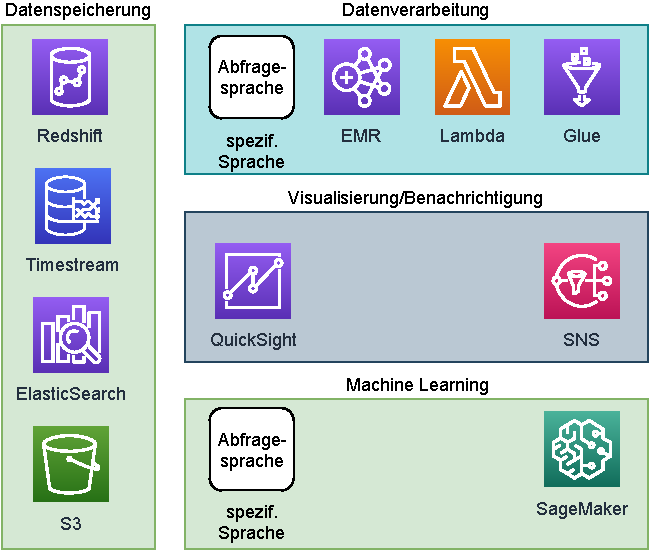
\includegraphics[width=\textwidth]{graphics/Overview-DB.pdf}
\caption{Einsetzbare Produkte im Bereich Datenbankverarbeitung}
\label{abb:ProdukteDB}
\end{figure}

\subsection{Amazon Timestream}
\lstset{language=SQL} 
\begin{lstlisting}
SELECT DeviceType,
  measure_name,
  BIN(time, 120m) AS binned_timestamp,
  ROUND(AVG(measure_value::double), 2) AS avg,
  ROUND(APPROX_PERCENTILE(measure_value::double, 0.99), 2) AS p99 
FROM "iot - demo".iot 
WHERE measure_name = 'temperature' 
  AND time > ago(24h) 
GROUP BY DeviceType,
  measure_name,
  BIN(time, 120m) 
ORDER BY ABS(avg - p99) DESC
\end{lstlisting}

\begin{table}[H]
\centering
\begin{tabular}{|l|l|l|l|l|}
\hline
DeviceType & measure\_name & binned\_timestamp & avg & p99 \\ \hline
iotDemo & temperature & 2021-02-26 08:00:00.000000000 & 16.51 & 20.1 \\ \hline
iotDemo & temperature & 2021-02-26 16:00:00.000000000 & 18.23 & 19.2 \\ \hline
iotDemo & temperature & 2021-02-25 18:00:00.000000000 & 18.5 & 19.3 \\ \hline
iotDemo & temperature & 2021-02-25 20:00:00.000000000 & 17.3 & 17.8 \\ \hline
\end{tabular}
\caption{Ausgabe der Datenbank bei Eingabe des oben gezeigten SQL-Statements}
\label{tab:AusgabeSQL}
\end{table}

\subsection{Amazon Redshift}

\subsection{Amazon MSK}

\subsection{Amazon Athena}

\subsection{Amazon Elasticsearch}

\subsection{Amazon S3}

\subsection{Produktauswahl}